\section{Myo armband overview} \label{sec:MYB}

The Myo armband (MYB) from Thalmic Labs will be used for EMG data acquisition. It contains eight dry stainless steel electrode-pairs around the inside of the armband, as depicted in \figref{fig:myoarmband}. The recorded EMG is unitless in an 8-bit resolution. As usual when recording EMG the higher the performed contraction is, the higher the float values in the output will be. To avoid interference from power lines a 50 Hz notch filter is implemented in the MYB. However, the MYB is not able to make any further filtering, thus this will be implemented later during signal processing described further in \secref{sec:prePros}. The MYB has a 200 Hz sample rate, and thus a lower resolution than the EMG spectrum \cite{Cram2012}. In \secref{Feature_extraction_meth}, different techniques to counter the negative effect of low-resolution EMG will be proposed for the implementation. Besides the EMG sensors the MYB can provide position and orientation information, using its three inertial measurement units consisting of a three axis gyroscope, a three axis magnetometer and a three axis accelerometer. This inertial information is sampled at 50 Hz. \cite{Myoarmband2013}

\begin{figure}[H]                 
	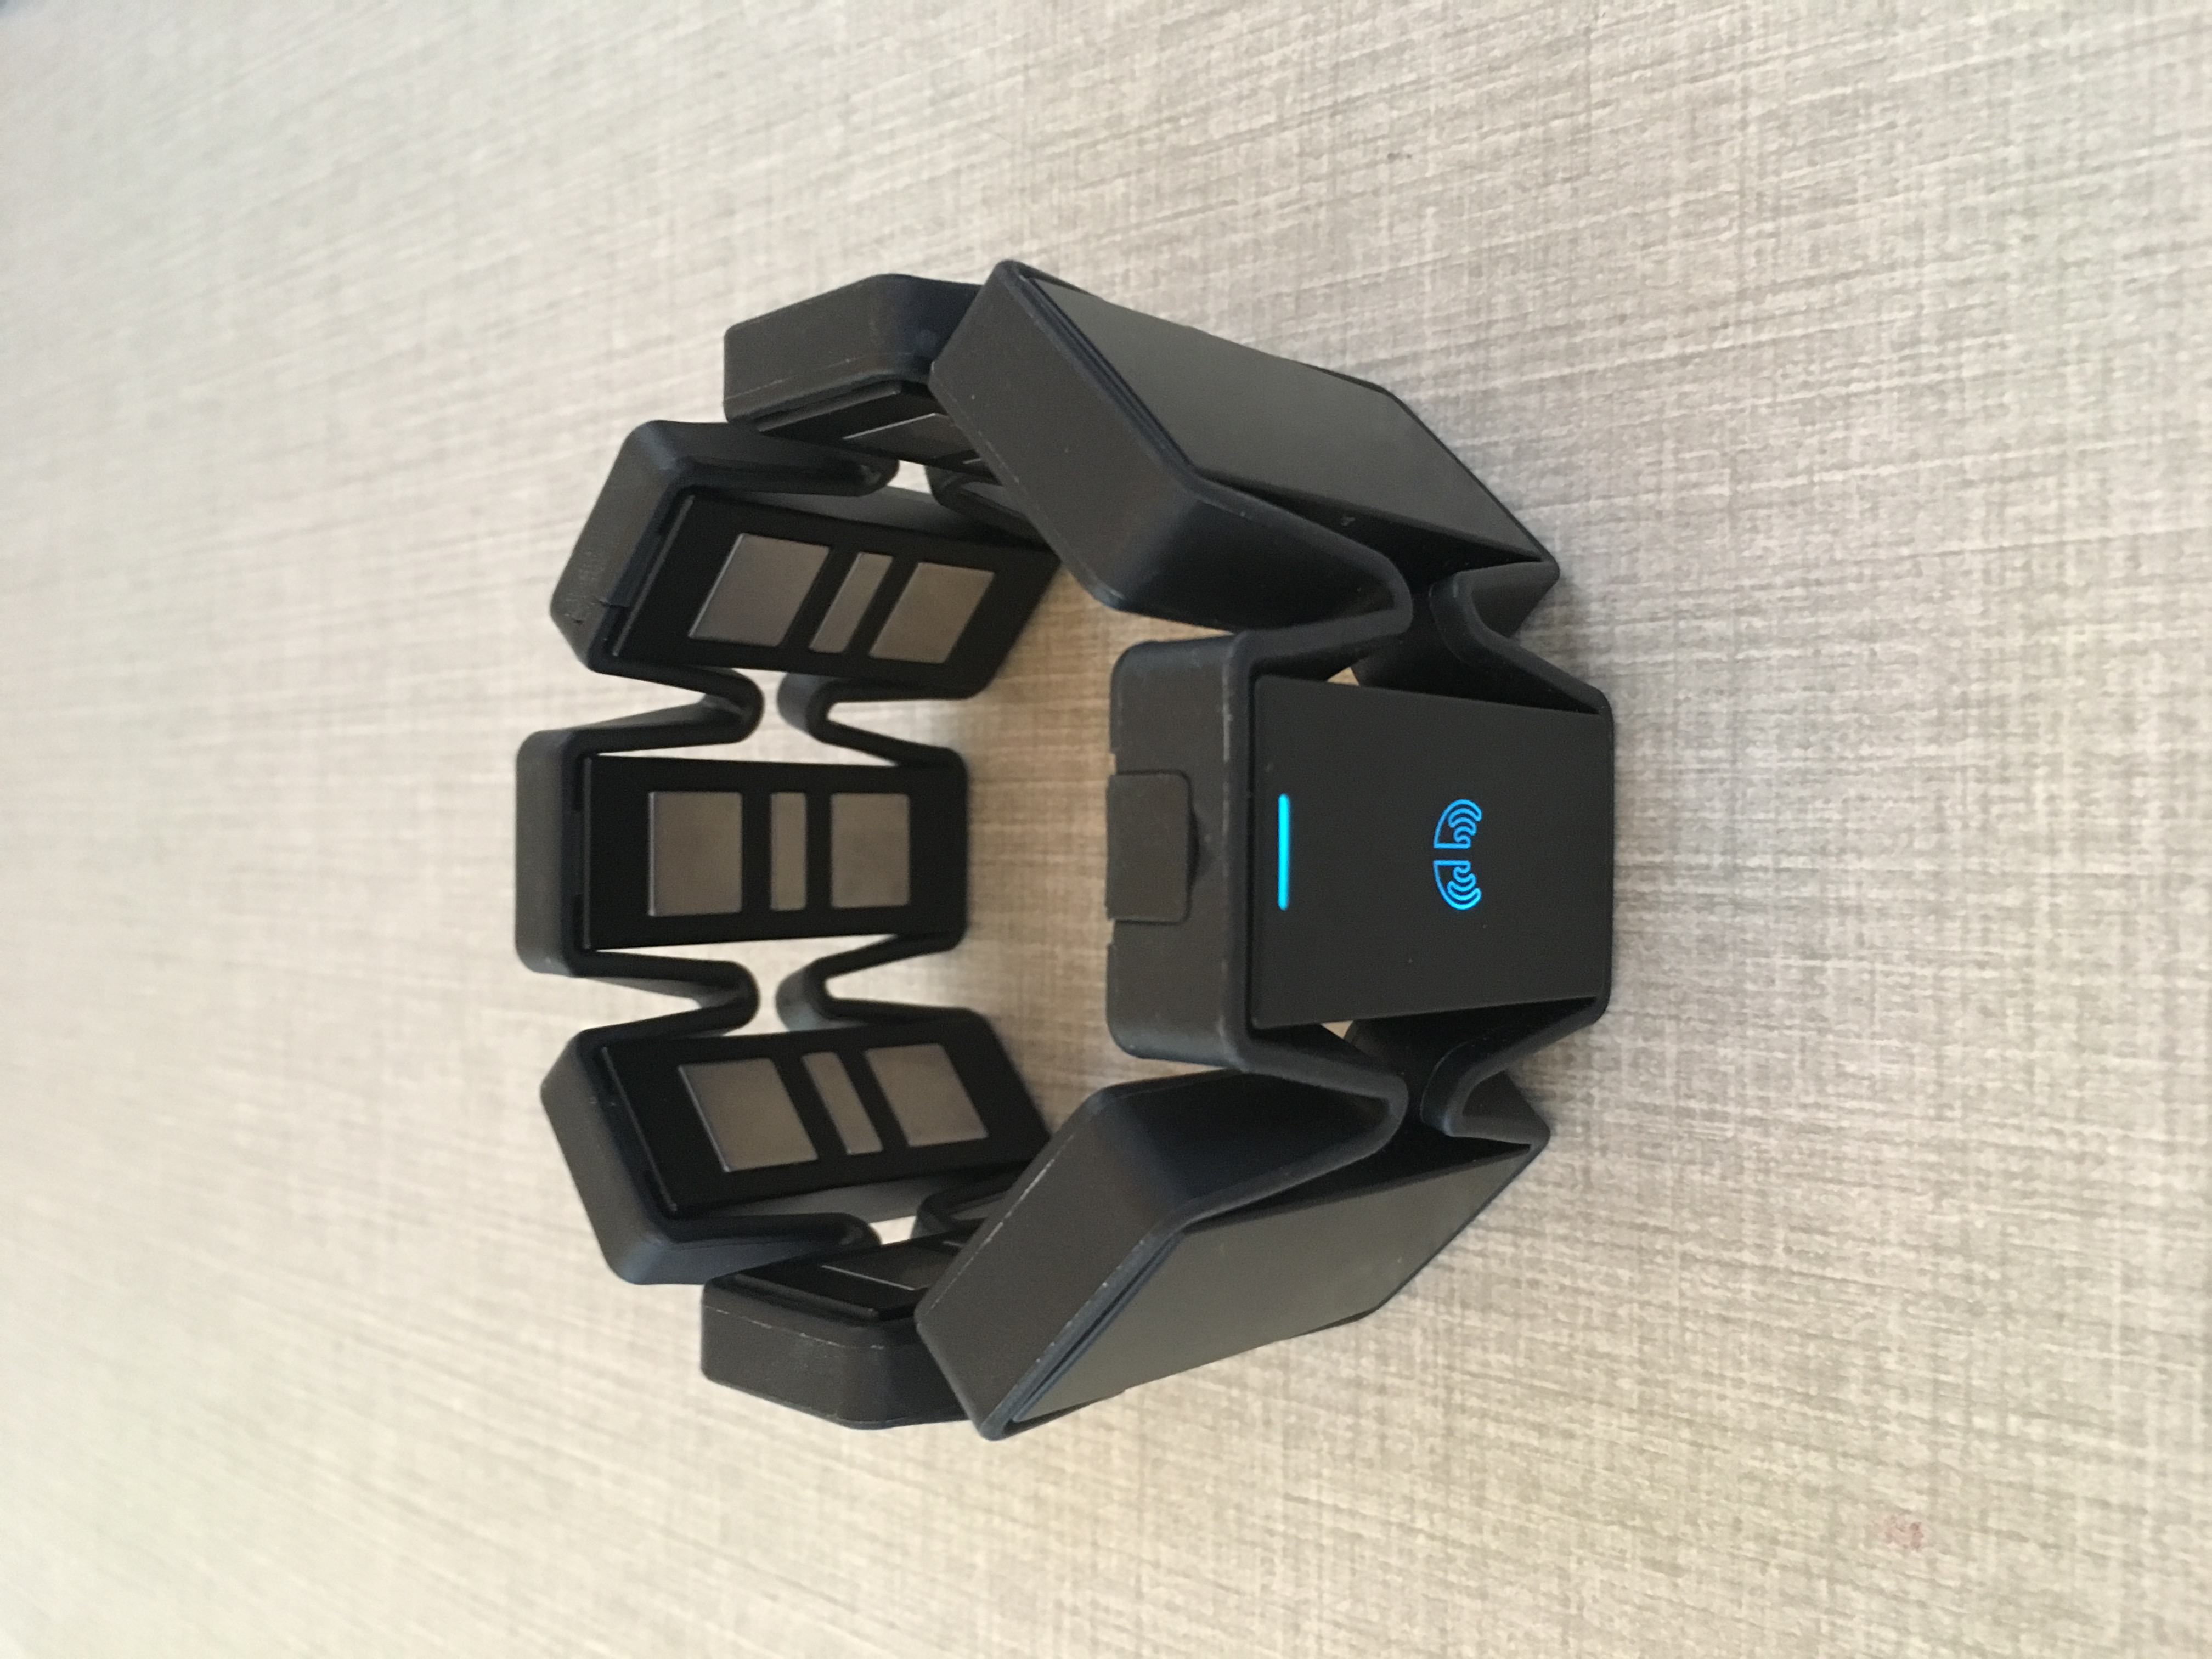
\includegraphics[width=.4\textwidth]{figures/xBackground/myoband}  
	\caption{MYB from Thalmic Labs. The number on each channel indicates which channel corresponds to which column in the digital output, when acquiring data from MYB.}
	\label{fig:myoarmband} 
\end{figure}

When initiating the wearing of the armband there is two calibration phases the user must follow before the armband is ready to use - the warm-up phase and the sync phase. During the warm-up phase the armband is ensuring a strong electrical connection with the muscles in the forearm as possible. This is mainly provided by light sweating on the skin under the electrodes, which improve the connection similar to electrode gel \cite{Cram2012}. During the sync phase, the armband determines its orientation in space, position on and which arm it is placed on. The MYB works better when fitted tightly on the thickest part of the forearm. For users with smaller forearms a set of clips can be added for the armband to get a constrained grip. \cite{Myoarmband2013}
